\documentclass[final]{anthology-ch}

\usepackage{booktabs}
\usepackage{graphicx}
\usepackage{pgfplots}
\usepackage{float}
\usepackage{longtable}

\pgfplotsset{compat=1.18}

\title{TrochAIc: Metrical Tools for AI Interpretability}

\author[1]{Ben Glaser}[
orcid=0009-0007-1079-9513
]

\affiliation{1}{Sterling Library and Poorvu Center for Teaching and Learning, Yale University, New Haven, CT, USA}

\keywords{LLMs, phonology, prosody, poetics, transformers}

\pubyear{2025}
\pubvolume{3}
\pagestart{1438}
\pageend{1453}
\conferencename{Computational Humanities Research 2025}
\conferenceeditors{Taylor Arnold, Margherita Fantoli, and Ruben Ros}
\doi{10.63744/K9Mwiiszu7QL}
\paperorder{89}

\addbibresource{bibliography.bib}

\begin{document}

\maketitle

\begin{abstract}
Versification has not been central to studies of AI poetry and poetic style. If we build tools to study the prosodic and phonological capacities of AI, we learn not just about AI verse but about  hidden histories of reception and genre. The computational humanities can unpack these histories and explain how LLMs reify a limited kind of poetry and language. We can also compile data to train models that behave differently. I share a >100K line data set of scanned 18\textsuperscript{th} century iambic pentameter, compare its versification with generative AI verse, and train BERT and T5 models with this data to scan meter and classify complexity. This tool lays the groundwork for exposing text-based LLMs to phonology and poetic prosody.
\end{abstract}

\section{Introduction}

Literary critics, computer scientists, and tech marketers alike have raised the specter of LLM poetry as a measure of linguistic robustness, intelligence, and even humanity. Recently, Porter and Machery \cite{porter_ai-generated_2024} published a highly visible and provocatively-titled essay “AI Generated Poetry is Indistinguishable from Human-Written Poetry and is Rated more Favorably,” with a computer scientists responding swiftly to observe their “staggering banality” \cite{davis_chatgpts_2024}.
\paragraph{}

Yet whether and how we find value in any poem is first a matter of literary theory and judgment. As Ryan Heuser succinctly puts it, “generative texts lack meaning not because they lack an author, but because they lack a context” \cite{heuser_generative_2025}. Porter and Machery collapse poetry into whatever can be produced and count as “poetry” in a context of their choosing. This repeats that lack of context, or what Michele Elam calls LLM’s “algorithmic ahistoricity” \cite{elam_poetry_2023}.
\paragraph{}

I argue that when we build tools to study the prosodic and phonological capacities of AI, we learn that AI poetry is not quite ahistorical. Rather, the sound (or silence) within their model of language reveals hidden histories of reception and genre. Elam further conceptualizes poetry as anathema to machine learning because it “will not optimize.” In what follows I ask how we might optimize LLMs for the uncharacteristic task of metrical scansion. I then show how computational humanities lets us refine data and train models that behave differently--though I make no claim as to the value or desirability of AI-generated verse itself. The real value, I argue, is in adding new tools to historical and formalist methods so we can manifest how mainstream LLMs reify a limited kind of poetry and language and, more importantly, improve our sense of what human poetry was and is.

\section{The Re-History of LLM Versification}

LLM poetry incessantly rhyme even when asked not to, constructing symmetrical iambic tetrameter about limited themes. A perfect storm of digitization, copyright, literary history, and choice of training tasks makes even advanced models sound like the uninventive 1890's  poets excoriated by modernists for heavily iambic rhythm. When asked to assess the value or function of meter, AI chatbots often use the adjective “sing-song,” as do many undergraduates before they learn formal analysis. GPTs retrace and cement one limited trajectory of literary meter.
\paragraph{}
We might think of the history of poetic meter not simply as a game of freedom and constraint, but as an implicit knowledge of English phonology made explicit to varying degrees as an abstraction into rules or constraints. The performance of LLMs does not reflect this history or knowledge. In the early twentieth century, with the rise of free verse and modernist ideologies of poetry, the diverse metrical techniques and theories of the long-nineteenth century became regimented and then rejected.\footnote{\cite{glaser_modernisms_2020}}  This winnowing of prosodic genres was a critical inflection point not just for poetry, but for literary criticism. LLM poetry generation and analysis bears the imprint of this transformation of historical prosody and its place in literary analysis. The rise of large scale natural language processing over the past four years thus extends the twentieth century’s reification of prosodic form. Prosody is viewed as and then becomes a mechanical task, and only a few such tasks turn out to be reproducible by AI.

\section{LLM Poetry's Task Structure}

McCoy et al. observe that Generative AI performs well on tasks they have either been trained to perform, or seen performed in data, but struggle to generalize from these \cite{mccoy_embers_2024}. McCoy gives the useful example of the internet-common letter cypher “Rot-13” (a --> n, b --> o, etc). LLMs can’t generalize “Rot-14”. A poetic analogue would be Haiku: LLMs can now be consistently prompted to produce a 5-7-5 syllabic pattern in English. Because counting syllables is an unusual and often difficult phonological task in English, and because LLMs do not “know” what a syllable is (without a separate program for counting), they cannot reliably create a 6-8-6 “Haiku+1,” or any of the myriad esoteric syllabic stanzas of the past 100 years (2-4-6-8-2 cinquains being quite popular between 1910-1930, but not at the digitized volume of reddit’s r/haiku).

\paragraph{}

It is unclear how LLMs can be trained to improve their syllabic intelligence. Daniel Von Strien has created a synthetic haiku dataset to perform DPO (Direct Preference Optimization) training of OpenHermes-2.5-Mistral-7b, creating “HaikuHermes.”\footnote{The training set and model can be viewed and deployed from https://huggingface.co/davanstrien/HaikuHermes-0.1-7B } Having been rewarded for producing 5 and 7 syllable chunks of text, this model is less likely to miscount syllables. Yet this is not a reproducible effort for prosodic form in general, as it relies heavily on easily scraped or generated synthetic data. More common is some form of instruction tuning. Porter and Machery’s prompt for GPT 3.5 to “Write a short poem in the style of [     ]” produces metrical quatrains with some evocative word choices. They give no discussion of alternate prompting strategies such as one or few-shot prompting or prompts that specify features of the poetry. Their singular prompt reflects a view of poetry as a genre of the proper name. Their study suggests that the public is not familiar with those genres (Dorothy Lasky is wonderful, but hardly a known style); they do however recognize poetry as a \textit{prosodic }genre of rhyming quatrains as well as a lexicon. The study therefore shows that “human-out-of-the-loop” prompting for a “short poem” maps one prosodic genre, the quatrain, with the proper name providing themes. The result is less stylometrics than sociology. It suggests more about a popular poetry literacy learned by LLMs.
\paragraph{}

Davis rejects the study on other grounds: AI’s “extremely limited technical toolbox.” Only AI-Shakespeare generates sonnet form, and AI-Dickinson alternates tetrameter and trimeter. Given that in neither case do the AI-poets produce anything like the target poet’s verse technique, but rather the “Shakespearian sonnet” and Dickinson’s most frequent hymnal stanza, this again confirms how LLMs succeed at tasks only when they align with easily abstracted prosodic genre. The closed loop of LLM training, prompting, and our assessment narrowly calibrates “poetry” into the prosodic genre of a vaguely English-American ballad stanza. If readers fail to see this narrowness, it is because they share a repertoire of prosodic genres restricted to gestures like the volta of a sonnet or the epigrammatic and Orientalized concision of the haiku.
\paragraph{}

One indicator of the kind of “instruction tuning” underpinning modern chatbot poetry is the dataset, method, and end-product “co-poet” designed by Chakrabarty et al. \cite{chakrabarty_help_2022}. Setting aside whether this collaborative tool has value for human poetry generation, or what such a tool \textit{should} look like, the project matters here because of the relationship between its \textit{synthetic} dataset and \textit{synthesized }instructions. The training data is \href{https://github.com/vishakhpk/creative-instructions}{open source}; here are a few characteristic examples from the 800k+ line training set \ref{tab:copoet_table}:

\begin{table}[h]
\centering

\begin{tabular}{| p{0.10\linewidth}  |p{0.35\linewidth} |p{0.35\linewidth}|}
\hline
Task & Prompt & Response \\
\hline
“Start / End” & Generate a poetic sentence about `parodies' and ending in `order' & Even in parodies ‚Äî there was order \\
\hline
“Haiku” & Write a haiku that includes the word `Military volunteer' & Donkey engineer / Military volunteer / celebrates new year \\
\hline
“Rhyme” & Write a poetic sentence that ends in a word which rhymes with `raise' & The eyes that fix you in a formulated phrase \\
\hline
Simile / Metaphor & Generate a metaphor about `canvas'

& The canvas is a patchwork \\
\hline

\end{tabular}
\caption{Training data for ``Co-Poet''}
\label{tab:copoet_table}
\end{table}

\paragraph{}
This training data format aligns the model with a composite approximation of some genre, superficially related to poetic genres. Aside from numerous local flaws in identifying poetic devices, what makes “co-poet” superficial at the macro level is the determination of genre by task, which attempts to remedy the model's fundamental abstraction from genre to word embeddings. Just as important as this macro level are the tasks that it leaves out: training in meter, stanzas beyond couplets, syntax, slant rhyme, lineation, allusion and other forms of figurative language.

\section{Formal Analysis of LLM Verse}

The narrowness of instruction-tuned “poetry” crystallizes in two new interdisciplinary analyses presented at NLP and Computational Humanities conferences in late 2024. In “Sonnet or Not, Bot? Poetry Evaluation for Large Models and Datasets,” Walsh et al., develop a test for ``how well LLMs can identify \textit{poetic form} for more than 20 poetic forms and formal elements'' \cite{walsh_sonnet_2024}.\footnote{They release a valuable database of annotated public domain poems with crucial metadata about where those poems appear in other training sets; this kind of work undoes the calculated opacity of much LLM training.} The study’s main conclusion is that a range of flagship LLMs classify “fixed poetic forms” better than “unfixed forms or formal elements.” The models struggle with longer “fixed forms” (villanelle, sestina, pantoums) compared to shorter (sonnet, ballad, haiku). The authors carefully note, however, that scholars in the digital humanities have long understood literary classification tasks as proof of the “fuzziness” or ambiguity of genre and formal concepts. Notably, the n=15 study of human classification attempts showed very poor performance, especially on a 13-line “haiku” that appears chosen despite lacking fixed syllable or line counts and not being identified by its author as a haiku.\footnote{Of “Poem Written with Buson,” Matthew Rohrer writes “I tried to write lines that sound a lot like them, while using lines of theirs that sound as modern as possible.” \url{https://www.poetryfoundation.org/poetrymagazine/articles/70164/authors-note-on-writing-with-basho-buson-and-issa }}
\paragraph{}
If both poetic genre and form are constitutively “fuzzy,”\footnote{On Clifford Geertz’s “blurred genres” and the “fuzziness” of form, see also  \cite{butterfield_fuzziness_2012}} and if, as Walsh et al. acknowledge, we struggle to know “whose versions of form will be reproduced” by LLMs, it is crucial to reflect on our “domain expertise” before further training and evaluating this new linguistic domain. The bigger problem, familiar to scholars of historical prosody, is that ``form'' as such does not delimit a coherent domain. The concept of poetic form both precedes and induces LLM’s “algorithmic ahistoricity.”\footnote{\cite{glaser_white_2024}}

\paragraph{}
Walsh et al’s second study, “Does ChatGPT have a Poetic Style,” seeks a more fine-grained analysis of form. Like the preceding study, they calibrate this analysis around the distinction between “fixed forms,” “formal elements,” and “unfixed forms” \cite{walsh_does_2024}. The latter are not forms, however, but various subgenres of lyric with varying prominence (there are 254 elegies but only 16 aubades in the dataset). Formal “elements” counted in the human corpus include 398 couplets, 89 quatrains, and 94 tercets. “Ballads” are not fixed forms but a diverse tradition with internal prosodic differences and national and historical divergences.

\paragraph{}
I believe that assessing AI classification of “style” requires the thing called “poetic form” because the latter looks like something we can annotate into training data. I do not think this is possible or useful at the chosen scale of genre. Efforts to classify form at scale—whether by humans or human AI trainers—is particularly susceptible to the statistical weakness Nan Z. Da identifies in many computational literary analyses: “To look for homologies in literature, (CLS) must eliminate much of high dimensional data and determine the top drivers of statistically significant variation” \cite{da_computational_2019}. LLMs are, poignantly, entire models of language built off a word-bag theory of language that substitutes the unique dimensions of literary data with orders of magnitude higher vector dimensionality that encodes only semantic value. Rather than follow prior machine learning strategies, we should critique them from a discipline specific understanding of what tokens and embeddings would need to look like. In other words, we should study LLMs as symptomatic of poor theories of poetry and literary language.
\paragraph{}

\section{Prosodic Analysis of LLM Verse}

To assess LLM style, I argue, requires the different scale represented by prosody: a scale that is in a sense both much bigger and much smaller. Studying meter is not, primarily, a classification task. Scansion’s goal is not to figure out the meter of a poem or line. Rather, it is to determine the line, poem, poet, and period’s techniques and how they relate to syntax, meaning, and genre functions. Neither of Walsh et al.'s pathbreaking studies define iambic meter beyond “a regular pattern of unstressed and stressed syllables,” although that is sufficient to observe that most GPT poetry is iambic. Walsh et al., suggest about 60\%, but Heuser and my own results below suggest it is close to 100\% unless one specifically prompts for free verse, haiku, and explicitly non-metrical verse (Walsh et al. observe “\textit{GPT-4’s increased ability to not produce iambic meter}”). Meter in these studies remains a proxy for genre or “form”; that may help one determine whether an LLM can escape its doggerel gravity well, but it tells us nothing about an LLM’s verse “style” at the level of the line, phrase, or word. Walsh et al. hint at a deeper level of stylistic detail when they note that “in” and “upon” are very common starting words in GPT-4 poems because they make it easy to write iambic rhythm. But the “iambic” label on its own tells us nothing about how syllable, groups of syllables, word stress, caesurae, intonational stress, and other aspects of prosodic phonology are represented within the latent space of LLMs. These elements are historically generative of English poetry (other languages have other phonologies and optimal meters).

\paragraph{}
When an LLM manages to produce prosodic structures, it is because those structures became generic enough at some point in digitized literary history to strongly correlate phonological patterns into sequences of words, i.e. concatenations. Shakespearian sonnets are the best example, but a scholar of nineteenth-century American poetry might be unsurprised that Claude excels at the Finnish Kalevala’s trochaic tetrameter of Longfellow’s bestselling 1855 \textit{Song of Hiawatha}. Stylometric analyses of LLM verse permits a new path to AI interpretability. At the same time, LLM’s prosodic {dys}fluency reminds us of the eccentricity of human language practices descirbed by Roman Jakobson’s “poetic function.”
\paragraph{}

Here I follow the work of Ryan Heuser, who compares frequency of syllable stress per metrical position in 10-syllable lines in LLMs and sonnets to find “mechanical regularity” that “exceeds even a rewinding of history from free verse to metrical tradition” \cite{heuser_generative_2025}. Using the scansion tool he developed with colleagues at Stanford, prosodic.py \cite{heuser_prosodic_2010}, I scanned >100k lines of iambic pentameter lines in the xml-formatted Eighteenth Century Poetry Archive (ECPA).\footnote{ECPA is an astonishing achievement of TEI, and I encourage readers to navigate to the site and see the xml encoding for themselves. \url{https://www.eighteenthcenturypoetry.org/works/bsb18-w0660.shtml}. I am grateful to its Alexander Huber and other developers. For my parsed data and full methodology including set of metrical constraints, see \url{https://github.com/cretic/metricalgpt/saved_corpora_parses/ECPA_data_and_parses/ecep_reparsed_full.csv}. }

\begin{figure}[H]
\centering
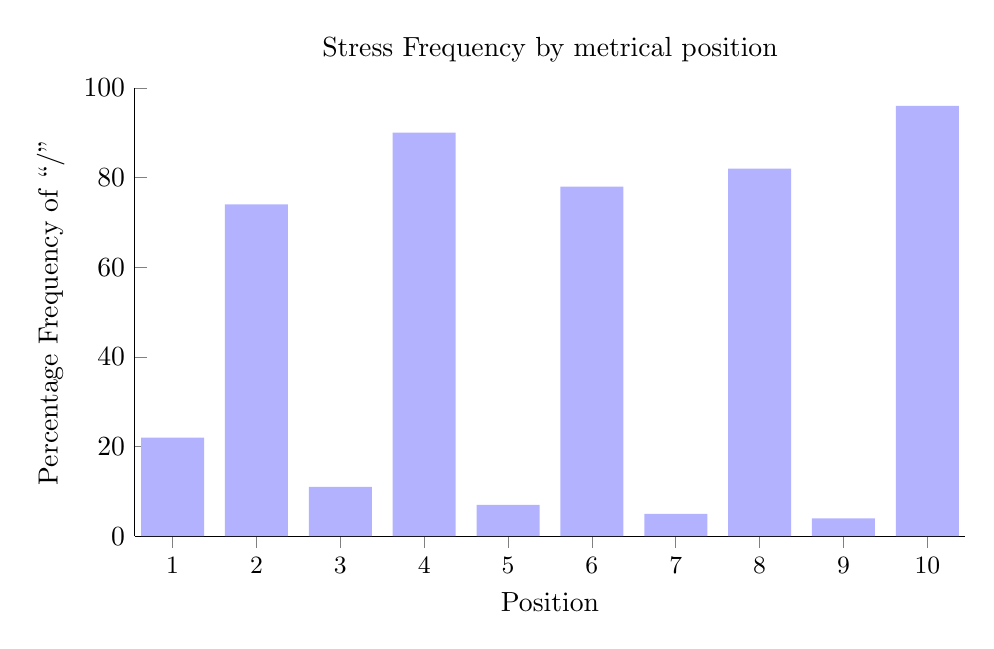
\begin{tikzpicture}
\begin{axis}[
ybar,
bar width=0.8cm,
width=\textwidth,
height=0.6\textwidth,
xlabel={Position},
ylabel={Percentage Frequency of ``/''},
title={Stress Frequency by metrical position},
ymin=0,
ymax=100,
ytick={0,20,40,60,80,100},
xtick=data,
xticklabels={ 1,  2,  3,  4,  5,  6,  7,  8,  9,  10},
x tick label style={rotate=0, anchor=north, font=\small},
enlarge x limits=0.05,
axis lines*=left,
ymajorgrids=false,
every axis plot/.append style={fill=cyan!60, draw=none}
]
\addplot coordinates {
(1, 22)
(2, 74)
(3, 11)
(4, 90)
(5, 7)
(6, 78)
(7, 5)
(8, 82)
(9, 4)
(10, 96)
};
\end{axis}
\end{tikzpicture}
\caption{Percentage frequency of / for each metrical position (pentameter)}
\label{fig:plus_frequency}
\end{figure}

\paragraph{}

Compare ChatGPT 4o’s performance when \textit{explicitly} prompted for variations like “trochaic inversion” (Figure \ref{fig:4o_stress_frequency}).
\paragraph{}

\begin{figure}[H]
\centering
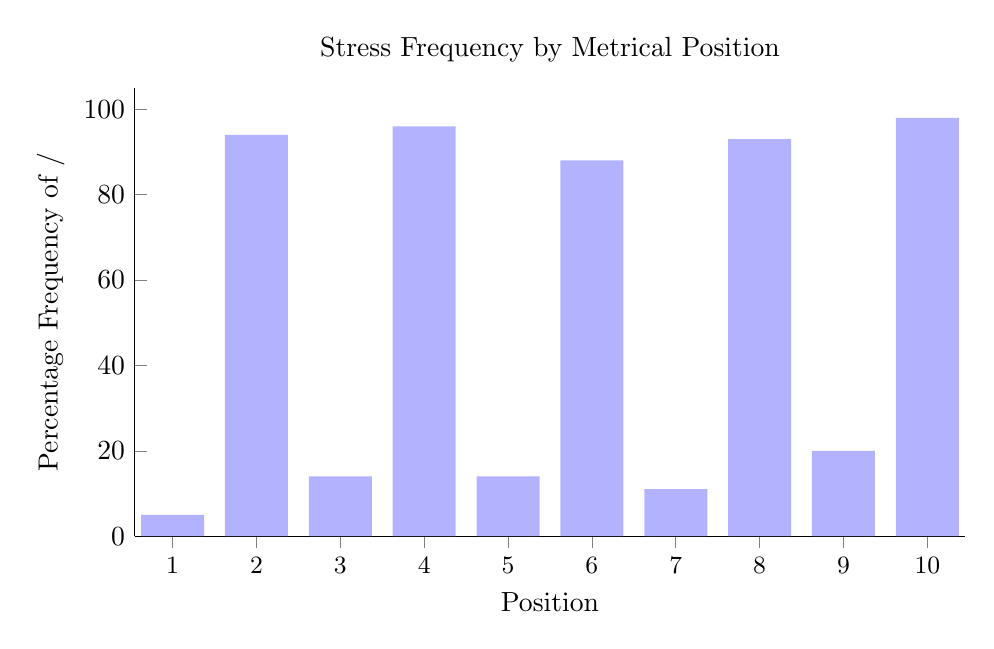
\begin{tikzpicture}
\begin{axis}[
ybar,
bar width=0.8cm,
width=\textwidth,
height=0.6\textwidth,
xlabel={Position},
ylabel={Percentage Frequency of /},
title={Stress Frequency by Metrical Position},
ymin=0,
ymax=105,
ytick={0,20,40,60,80,100},
xtick=data,
xticklabels={ 1,  2,  3,  4,  5,  6,  7,  8,  9,  10},
x tick label style={rotate=0, anchor=north, font=\small},
enlarge x limits=0.05,
axis lines*=left,
ymajorgrids=false,
every axis plot/.append style={fill=cyan!60, draw=none}
]
\addplot coordinates {
(1, 5)
(2, 94)
(3, 14)
(4, 96)
(5, 14)
(6, 88)
(7, 11)
(8, 93)
(9, 20)
(10, 98)
};
\end{axis}
\end{tikzpicture}
\caption{Percentage frequency of / for each metrical position (pentameter)}
\label{fig:4o_stress_frequency}
\end{figure}

Such regularity is far in excess of any historical practice, as hand counted by Marina Tarlinskaja, and particularly skewed in the first two positions:

\begin{table}[H]
\centering
\begin{tabular}{|c|c|l|l|l|l|l|}
\hline
Positions& 2& 4& 6& 8& 10&Mean 2-8\\
\hline
Pope& 78& 98& 74& 86& 99&84\\\hline
Byron& 71& 80& 76& 70& 94&74\\\hline
Shakespeare& 61& 82& 73& 69& 93&71\\
\hline
Frost& 61& 79& 75& 74& 94&72\\\hline
Donne& 61& 80& 67& 71& 78&70\\\hline
10-syllable prose& 38& 40& 48& 38& 80&48\\ \hline
\end{tabular}
\caption{Tarlinskaja, Stress in Even Positions \cite{tarlinskaja_what_2006}}
\label{tab:example}
\end{table}

A more fine-grained analysis of rhythmical “figures,” i.e. specific stress contours employed historically to draw attention and delight, shows even more mechanicity. For example, the rhythmic figure /xx/, sometimes called a ``trochaic inversion'' or ``inverted foot,'' occurs in about 30\% of eighteenth-century blank verse lines, usually at the start of the line. Yet prompting for such variation paradoxically decreases frequency of /xx/ (Figure \ref{fig:/xx/_variation}).

\begin{figure}[h]
\centering
\scalebox{.8}{
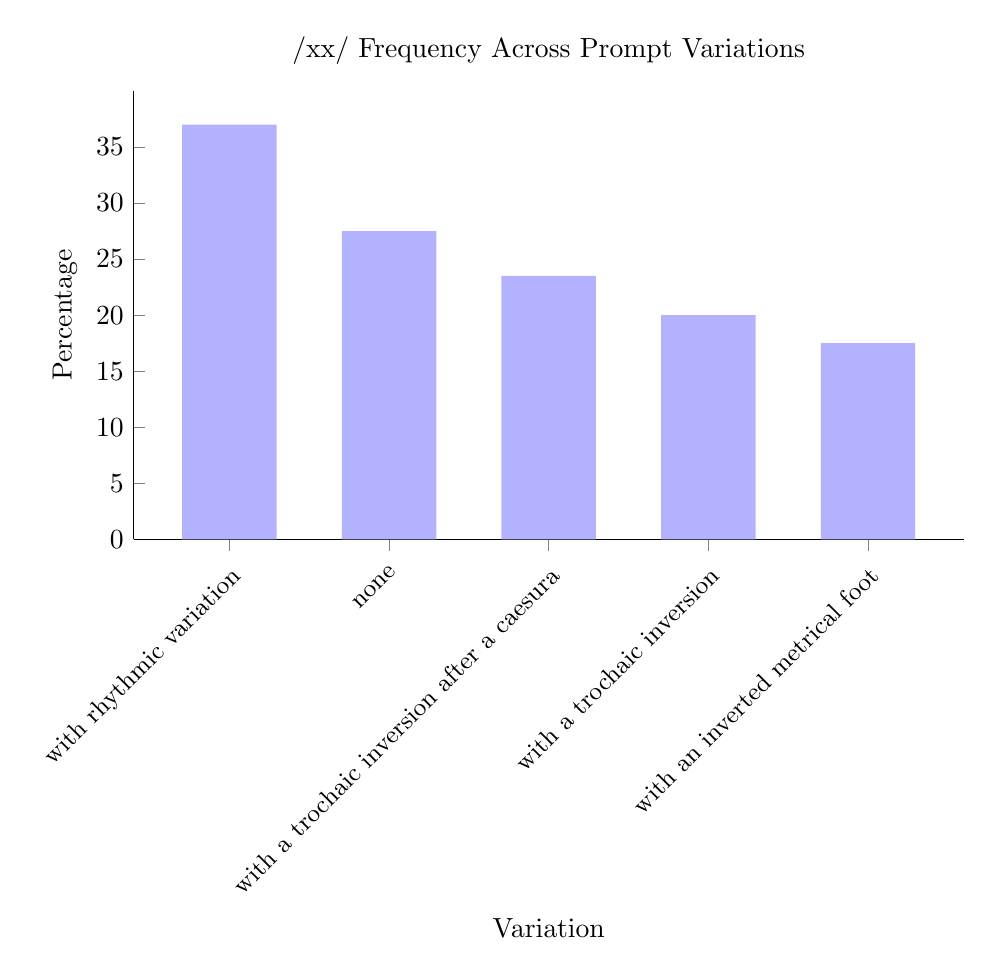
\begin{tikzpicture}
\begin{axis}[
ybar,
bar width=1.2cm,
width=\textwidth,
height=0.6\textwidth,
xlabel={Variation},
ylabel={Percentage},
title={/xx/ Frequency Across Prompt Variations},
ymin=0,
ymax=40,
ytick={0,5,10,15,20,25,30,35},
xtick=data,
symbolic x coords={with rhythmic variation, none, with a trochaic inversion after a caesura, with a trochaic inversion, with an inverted metrical foot},
x tick label style={rotate=45, anchor=north east, font=\small},
enlarge x limits=0.15,
axis lines*=left,
ymajorgrids=false,
every axis plot/.append style={fill=cyan!60, draw=none}
]
\addplot coordinates {
(with rhythmic variation, 37)
(none, 27.5)
(with a trochaic inversion after a caesura, 23.5)
(with a trochaic inversion, 20)
(with an inverted metrical foot, 17.5)
};
\end{axis}
\end{tikzpicture}
}
\caption{/xx/ frequency in GPT 4o}
\label{fig:/xx/_variation}
\end{figure}

If we look at the rhythmic figure “xxx,” i.e. three unstressed positions, we see something even more striking: this figure appears in \textbf{41\% }of ECPA lines, and only ~5\% of GPT 4o's blank verse (Figure \ref{fig:www_variation}). This shows us that human poets tend towards a lighter line, often one with four stresses total, as a natural consequence of English phonology and the many function words (to, a, in) on which syntax relies after grammatical case was lost. LLMs lack this attention to natural language stress once prompted for poetry and especially when prompted for meter of any sort. The key finding here is that prompting (and likely any form of instruction tuning) will not produce metrical complexity. The enormous diversity of verse technique compared to LLM’s few species of rigid meter suggests both the obvious absence of phonological awareness and the more interesting presence of prompt frameworks and fine-tunings that pull anything prosody related toward one or two rhythmic patterns.
\paragraph{}

\begin{figure}[h]
\centering
\scalebox{.8}{
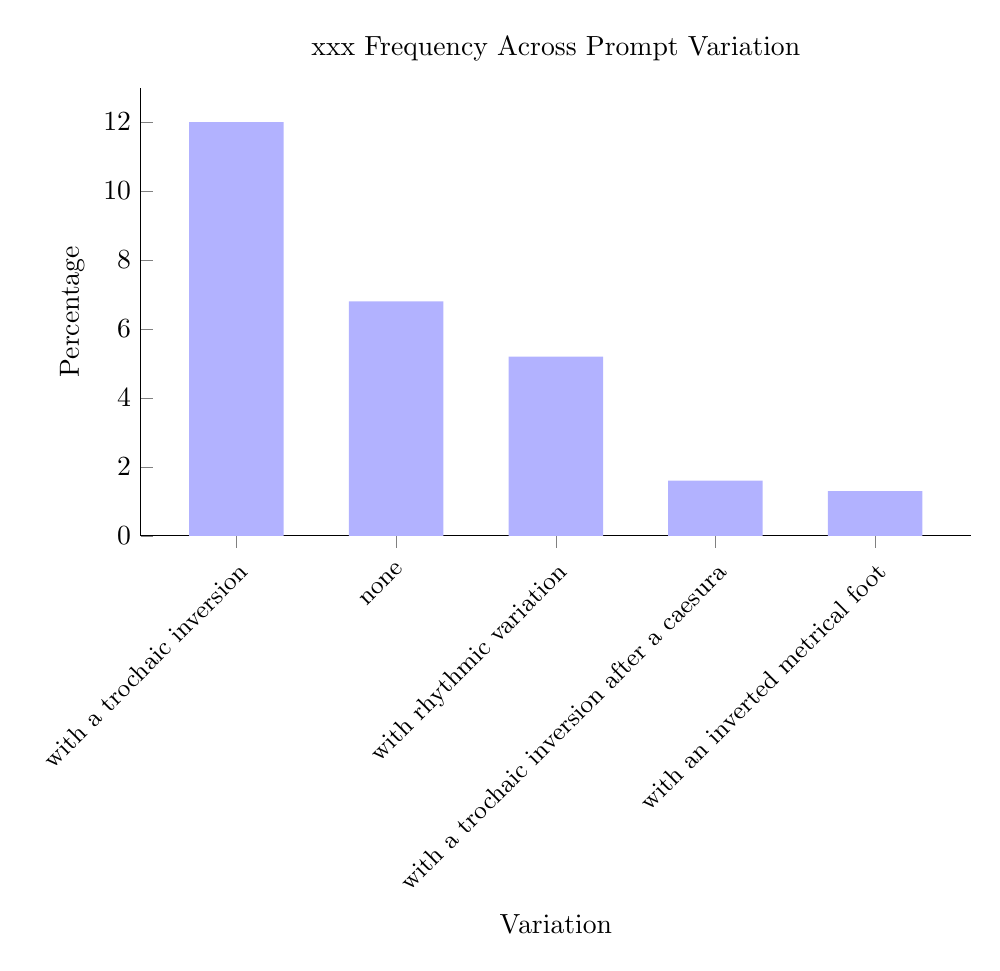
\begin{tikzpicture}
\begin{axis}[
ybar,
bar width=1.2cm,
width=\textwidth,
height=0.6\textwidth,
xlabel={Variation},
ylabel={Percentage},
title={xxx Frequency Across Prompt Variation},
ymin=0,
ymax=13,
ytick={0,2,4,6,8,10,12},
xtick=data,
symbolic x coords={with a trochaic inversion, none, with rhythmic variation, with a trochaic inversion after a caesura, with an inverted metrical foot},
x tick label style={rotate=45, anchor=north east, font=\small},
enlarge x limits=0.15,
axis lines*=left,
ymajorgrids=false,
every axis plot/.append style={fill=cyan!60, draw=none}
]
\addplot coordinates {
(with a trochaic inversion, 12)
(none, 6.8)
(with rhythmic variation, 5.2)
(with a trochaic inversion after a caesura, 1.6)
(with an inverted metrical foot, 1.3)
};
\end{axis}
\end{tikzpicture}
}
\caption{xxx frequency in GPT 4o}
\label{fig:www_variation}
\end{figure}

%\newpage
\section{Training Experiments}

To move from simple analysis of decoder models' output to encoding prosodic features required substantial data collection and curation and symbolic representations of prosody (scansions). First, however I tested what might happen with purely text-based fine-tuning on unusually divergent and complex metrical poetry. Could one push models out of their iambic comfort zone?

\subsection{John Milton's Twin}

Compare the following two versions of gemini flash-1.5. On the left, a fine-tuned model trained to generate lines from Paradise Lost. The training data here is 1000 pairings of input=line n, output=line n+1. In other words, if given ``Of man's first disobedience, and the fruit,'' gemini tries to produce ``of that forbidden tree, who mortal taste.'' What metrical system, if any, would be induced? The result was surprising. Next to the fine-tuned model is an un-tuned model given only the system prompt ``You are the poet John Milton. When the user inputs a line, you write the next line in Milton's blank verse.'' The output becomes the next input. Early modernists and prosodists may recognize the rhythmic divergence in caesura location (color coded).

\paragraph{}

\begin{figure}[H]
\centering
\includegraphics[width=1\linewidth]{figures/miltonbots.png}
\label{fig:miltonbots}\caption{Gemini flash 1.5, Fine-tuned vs Prompted. Red marks odd-positioned caesurae or strong phrase boundaries; green marks even ones. August 2024 }
\end{figure}

Where Milton performs systematic irregularity, LLMs get stuck dividing their lines after the fourth syllable (with pause or phrasal boundary). The tuned model enjambs, the un-tuned model always endstops. The metrical diversity may be a function of Milton's syntax, the way he concatenates phrases, and a liberation from the requirement that the line rather than the sentence frame the unit of sense. This was Milton's central innovation in versification, and here it has the knock-on effect of rhythmical flexibility. Notably, the tuned Milton maintains decasyllabic metricality, suggesting that an LLM may encode these through pure word sequencing constraints.

\subsection{metricalBERT}

\paragraph{}

The first challenge of training LLM attention on prosody is the absence of formatted data that includes metrical structure. Inspiration could come from using an analogue of \href{https://microsoft.github.io/muzic/musicbert/}{musicBERT} to create higher-dimensional tokens including metrical information and phonological representation (IPA or CMUDict encodings). One could otherwise concatenate prosodic data as part of the tokenization process. For example, PoeLM (2022) prepends syllable count and rhyme as control codes.\footnote{https://aclanthology.org/2022.findings-emnlp.268/} The creators tag non-verse texts with its syllable count and rhyme to train a model and then control the structure of generated text. Yet only limited efforts have been made to “concatenate tonal information to the character embeddings of an LSTM to create a model that is more phonologically compliant.” No one has done this for accentual-syllabic poetry and English, which present major complications because of complex and hierarchical stress structures.\footnote{Another model, poet-vicuna-13B, works by constraining token choice to avoid running over max syllable count (“a logit warper that constrains model vocabulary during the generation process”). See \url{https://github.com/joehoover/cog-poet-vicuna-13b}. Yet logit warpers modify only the probabilistic process; they are not the same as lexical choice according to qualitative constraints. They show that there is little value in post-embedding layers as “mechanisms for constrained generation” such as forcing syllable counting for “proper metric patterns (e.g. iambic pentameter for our readers who know their scansion).”}
\paragraph{}

To compile phonological data for LLM training, I deployed prosodic.py at scale on the ECPA corpus. The result is a >100k line database of scanned iambic pentameter, including a symbolic representation of both stress pattern (rhythm), meter (underlying structure), and a quantitative measure of complexity.\footnote{\url{https://huggingface.co/datasets/bensglaser/18C_IP_Scanned}} Using only the data on metrical complexity, I first fine-tuned several BERT classification models. These indicate a modest potential for inducing metrical awareness into a text-only transformer model. Here is a confusion matrix for ``metricalBERT\_0\_2\_4,'' trained on the scanned ECPA corpus to predict a line's metrical complexity as either 0 (simple, no tension), 2, or 4 (a fairly high degree of complexity). Accuracy reached 75\%.\footnote{My training of BERT models was supported by Katelyn DeKeersgieter. The model is available at \url{https://huggingface.co/katelyndekeer/metricalBERT_0_2_4}}

\begin{figure}[H]
\centering
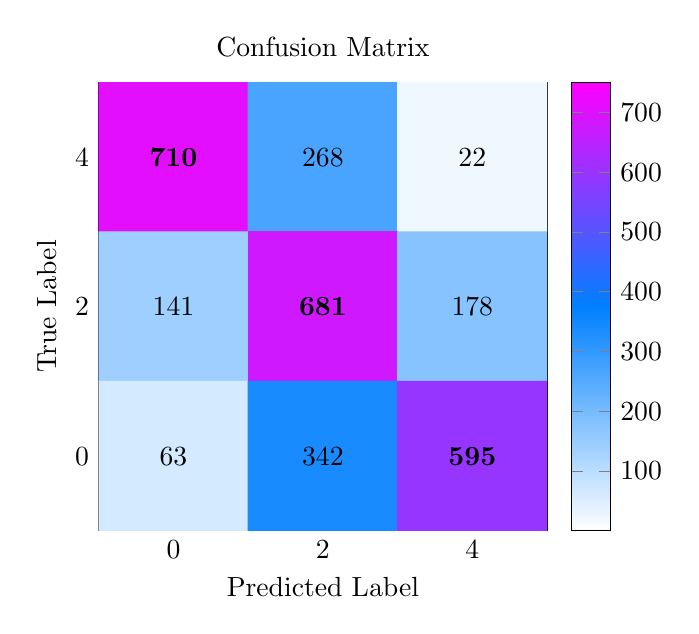
\begin{tikzpicture}
\begin{axis}[
colormap/cool,
colorbar,
colorbar style={
ylabel={},
ytick={100,200,300,400,500,600,700},
},
xlabel={Predicted Label},
ylabel={True Label},
title={Confusion Matrix},
xtick={0,1,2},
xticklabels={0,2,4},
ytick={0,1,2},
yticklabels={0,2,4},
enlargelimits=false,
axis equal image,
width=0.6\textwidth,
height=0.6\textwidth,
point meta min=0,
point meta max=750,
]
\addplot[
matrix plot*,
mesh/cols=3,
point meta=explicit,
] table[meta=C] {
x y C
0 2 710
1 2 268
2 2 22
0 1 141
1 1 681
2 1 178
0 0 63
1 0 342
2 0 595
};

\node at (axis cs:0,2) {\textbf{710}};
\node at (axis cs:1,2) {268};
\node at (axis cs:2,2) {22};
\node at (axis cs:0,1) {141};
\node at (axis cs:1,1) {\textbf{681}};
\node at (axis cs:2,1) {178};
\node at (axis cs:0,0) {63};
\node at (axis cs:1,0) {342};
\node at (axis cs:2,0) {\textbf{595}};
\end{axis}
\end{tikzpicture}
\caption{MetricalBERT 0/2/4 Confusion matrix}
\label{fig:confusion_matrix}
\end{figure}

A purely binary version (0 or 3) approached 80\% accuracy.\footnote{https://huggingface.co/katelyndekeer/binary\_metricalBERT} The most promising model, “trochaicBERT”, was trained on the ECPA corpus to differentiate between the 30k lines that have the rhythmic figure “/xx/” (a kind of metrical inversion, sometimes called a trochaic “foot”) and the 70k that do not.\footnote{https://huggingface.co/bensglaser/trochaic\_bert} Here precision approached 90-95\%\ (Figure \ref{fig:trochaic_confusion_matrix}).

\begin{figure}[H]
\centering
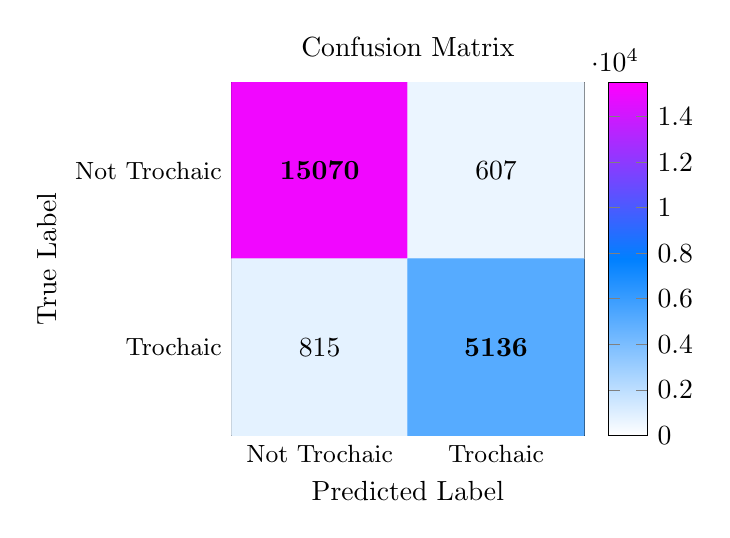
\begin{tikzpicture}
\begin{axis}[
colormap/cool,
colorbar,
colorbar style={
ylabel={},
ytick={0,2000,4000,6000,8000,10000,12000,14000},
},
xlabel={Predicted Label},
ylabel={True Label},
title={Confusion Matrix},
xtick={0,1},
xticklabels={Not Trochaic, Trochaic},
ytick={0,1},
yticklabels={Trochaic, Not Trochaic},
x tick label style={font=\small},
y tick label style={font=\small},
enlargelimits=false,
axis equal image,
width=0.5\textwidth,
height=0.5\textwidth,
point meta min=0,
point meta max=15500,
]
\addplot[
matrix plot*,
mesh/cols=2,
point meta=explicit,
] table[meta=C] {
x y C
0 1 15070
1 1 607
0 0 815
1 0 5136
};

\node at (axis cs:0,1) {\textbf{15070}};
\node at (axis cs:1,1) {607};
\node at (axis cs:0,0) {815};
\node at (axis cs:1,0) {\textbf{5136}};
\end{axis}
\end{tikzpicture}
\caption{Confusion matrix of trochaicBERT's classification results.}
\label{fig:trochaic_confusion_matrix}
\end{figure}

\subsection{metricalT5}

metricalBERT showed how classifiers trained on curated prosodic data add phonological information to embeddings of poetic lines. To test the downstream generation and sequence to sequence capacity of transformers, I tagged the dataset to train Google's T5\_large encoder-decoder model using an input-output format. This tracks with the method of training in \cite{walsh_sonnet_2024} and \cite{chakrabarty_help_2022}, relying on annotated datasets converted into sequence transformation tasks in tandem with previously discussed numerical classification of complexity. Prior to this training, I refined our ECPA scansion using openrefine. This removed approximately 2k poorly scanned lines including residual tetrameter and hexameter. To better account for how prosodic.py scores the complexity of lines with uncommon meters, I summed prosodic.py's score for metrical tension with the Levenshtein distance between the meter prosodic.py assigns and the normative and most common pattern WSWSWSWSWS. Accounting for complexity, which ultimately involves a degree of subjectivity and subtlety, is a work in progress. The more complex, the less rigorous, as perhaps indicated by the confusion matrix in Figure \ref{fig:complexity_confusion_matrix}.

\begin{table}[H]
\centering
\begin{tabular}{|p{0.50\linewidth}  |p{0.35\linewidth }|}

\hline
Input & Target \\
\hline
transform to meter: What fully to describe is past my Art; & WSWSWSWSWS \\
\hline
transform to rhythm: What fully to describe is past my Art; & x/xxx/x/x/ \\
\hline
predict complexity: What fully to describe is past my Art; & 1 \\
\hline
transform to meter: Faint as a chicken's note that has the pip: & SWWSWSWSWS \\
\hline
transform to rhythm: Faint as a chicken's note that has the pip: & /xx/x/x/x/ \\
\hline
predict complexity: Faint as a chicken's note that has the pip: & 2 \\
\hline

\end{tabular}
\caption{Sample training data for metricalT5}
\label{tab:t5_training_table}
\end{table}

\begin{figure}
\centering
\includegraphics[width=0.75\linewidth]{figures/complexity_confusion_matrix_normalized.png}
\caption{metricalT5 Complexity Confusion Matrix}
\label{fig:complexity_confusion_matrix}
\end{figure}

MetricalT5 achieved high precision (93\%) oon the ``predict complexity'' task. It also performs extremely well on sequence transformations, achieving 96\% accuracy on both ``transform to meter'' and ``transform to rhythm''.\footnote{Performance data is available at \url{https://huggingface.co/bensglaser/metricalT5-large/blob/main/1000line_rhythm_meter_test.csv}} Figure \ref{tab:t5_rhythm_transform} provides two of the 958 rhythm matches and two of the 42 mismatches. MetricalT5's predictions could facilitate corpus level search and analysis of prosody, for example recurrent rhythmic patterns. It could also guide future LLMs to optimize for more complex and diverse metrical patterns. There are several limitations here, however. Human annotation will always diverge in individual cases; moving outside 18th century poetry and encountering novel words will diminish results; the model has no ability at present to scan non-iambic pentameter lines. It is not, at present, a good tool for the study of individual lines, much less a replacement for teaching and performing (human) scansion.

\begin{table}[H]
\centering
\begin{tabular}{|p{0.45\linewidth}  |p{0.20\linewidth } |p{0.20\linewidth }|p{0.10\linewidth }|}

\hline
Input & Target & Predicted & Match\\

\hline
transform to rhythm: Unseen its progress, but its power you find;	& x/x//xx/xx/	& x/x//xx/xx/ & True \\
\hline
transform to rhythm: Is never with impunity defied. & x/xxx/xxx/ & x/xxx/xxx/ & True \\
\hline
transform to rhythm: Versailles appears --  its painted galleries, &	x/x/x/x/xx	& x/xxx/x/xx	& False \\
\hline
transform to rhythm: Let Vales embroidery wear, let Flowers be tinged & //x/xx///x// & //x/xx///xx/ & False \\
\hline

\end{tabular}
\caption{metricalT5 rhythm transform}
\label{tab:t5_rhythm_transform}
\end{table}

Finally, I provide a comparative analysis of Shakespeare's Sonnet 129 using metricalT5, prosodic.py with human emendations, and a few-shot prompting of Claude's Sonnet 4.5 model. For Claude, I provided a scansion of Sonnet 116 and the prompt ``You are a poetry scholar who scans lines of poetry to determine 1) their underlying metrical pattern, 2) the stress pattern of their performance, and 3) the complexity of the line. Complexity is a function of the distance between (1) and (2).'' As with the ECPA training data I regularized spelling. Error distance is measured via Levenshtein distance, namely how many character edits are required to match values. A unified table of these results is available at \url{https://github.com/cretic/t5-metrical-poetry}.

\begin{table}[htbp]
\centering
\small
\resizebox{\textwidth}{!}{%
\begin{tabular}{lp{0.8\textwidth}}
\toprule
\# & line \\
\midrule
1 & The expense of spirit in a waste of shame \\

2 & Is lust in action; and till action, lust \\

3 & Is perjured, murderous, bloody, full of blame, \\

4 & Savage, extreme, rude, cruel, not to trust, \\

5 & Enjoyed no sooner but despised straight, \\

6 & Past reason hunted; and, no sooner had \\

7 & Past reason hated as a swallowed bait \\

8 & On purpose laid to make the taker mad; \\

9 & Mad in pursuit and in possession so, \\

10 & Had, having, and in quest to have, extreme; \\

11 & A bliss in proof and proved, a very woe; \\

12 & Before, a joy proposed; behind, a dream. \\

13 & All this the world well knows; yet none knows well \\

14 & To shun the heaven that leads men to this hell. \\
\bottomrule
\end{tabular}
}
\caption{Shakespeare Sonnet 129}
\label{tab:poem}
\end{table}

\begin{table}[htbp]
\centering
\small
\resizebox{\textwidth}{!}{%
\begin{tabular}{lccccc}
\toprule
\# & prosodic complexity & t5 complexity & claude complexity & t5 error & claude error \\
\midrule
1 & 2.0 & 2.0 & 1.0 & 0.0 & 1.0 \\
\hline
2 & 1.0 & 1.0 & 1.0 & 0.0 & 0.0 \\
\hline
3 & 0.0 & 3.0 & 1.0 & 3.0 & 1.0 \\
\hline
4 & 4.0 & 5.0 & 3.0 & 1.0 & 1.0 \\
\hline
5 & 2.0 & 3.0 & 2.0 & 1.0 & 0.0 \\
\hline
6 & 3.0 & 3.0 & 4.0 & 0.0 & 1.0 \\
\hline
7 & 2.0 & 2.0 & 3.0 & 0.0 & 1.0 \\
\hline
8 & 0.0 & 0.0 & 0.0 & 0.0 & 0.0 \\
\hline
9 & 2.0 & 2.0 & 2.0 & 0.0 & 0.0 \\
\hline
10 & 1.0 & 1.0 & 4.0 & 0.0 & 3.0 \\
\hline
11 & 0.0 & 0.0 & 2.0 & 0.0 & 2.0 \\
\hline
12 & 0.0 & 0.0 & 0.0 & 0.0 & 0.0 \\
\hline
13 & 3.0 & 4.0 & 1.0 & 1.0 & 2.0 \\
\hline
14 & 2.0 & 2.0 & 1.0 & 0.0 & 1.0 \\
\hline
average error &  &  &  & 0.429 & 0.929 \\
\bottomrule
\end{tabular}
}
\caption{Complexity Analysis: T5 vs Claude}
\label{tab:complexity}
\end{table}

\begin{table}[htbp]
\centering
\small
\resizebox{\textwidth}{!}{%
\begin{tabular}{cccccc}
\toprule
Line & Prosodic Meter & T5 Meter & T5 Lev Dist & Claude Meter & Claude Lev Dist \\
\midrule
1 & WWSWSWSWSWS & WWSWSWSWSWS & 0.0 & WSWSWSWSWS & 1.0 \\
2 & WSWSWSWSWS & WSWSWSWSWS & 0.0 & WSWSWSWSWS & 0.0 \\
3 & WSWSWSWSWS & WSWSWWSWSWS & 1.0 & WSWSWSWSWS & 0.0 \\
4 & SWWSWSWSWS & SWWSWSWSWS & 0.0 & SWSWSWSWWS & 2.0 \\
5 & WSWSWSWSWS & WSWSWSWSWS & 0.0 & WSWSWSWSWS & 0.0 \\
6 & WSWSWSWSWS & WSWSWSWSWS & 0.0 & SWSWSWSWWS & 2.0 \\
7 & WSWSWSWSWS & WSWSWSWSWS & 0.0 & SWSWSWSWWS & 2.0 \\
8 & WSWSWSWSWS & WSWSWSWSWS & 0.0 & WSWSWSWSWS & 0.0 \\
9 & WSWSWSWSWS & WSWSWSWSWS & 0.0 & SWSWSWSWSW & 2.0 \\
10 & WSWSWSWSWS & WSWSWSWSWS & 0.0 & SWSWSWSWSW & 2.0 \\
11 & WSWSWSWSWS & WSWSWSWSWS & 0.0 & WSWSWSWSWW & 1.0 \\
12 & WSWSWSWSWS & WSWSWSWSWS & 0.0 & WSWSWSWSWS & 0.0 \\
13 & WSWSWSWSWS & SWWSWSWSWS & 2.0 & WSWSWSWSWS & 0.0 \\
14 & WSWSWSWSWWS & WSWSWSWSWS & 1.0 & WSWSWSWSWS & 1.0 \\
average distances &  &  & 0.286 &  & 0.929 \\
\bottomrule
\end{tabular}
}
\caption{Meter Analysis: T5 vs Claude} 
\label{tab:meter}
\end{table}

\begin{table}[htbp]
\centering
\small
\resizebox{\textwidth}{!}{%
\begin{tabular}{cccccc}
\toprule
Line & Prosodic Rhythm & T5 Rhythm & T5 Lev Dist & Claude Rhythm & Claude Lev Dist \\
\midrule
1 & xx/x/x/x/x/ & xx/x/x/x/x/ & 0.0 & x/xx/xx/x/ & 3.0 \\
2 & x/x/xxx/x/ & x/x/xxx/x/ & 0.0 & x/xx/x/x/x/ & 2.0 \\
3 & x/x/x/x/x/ & x/x/xx/x/x/ & 1.0 & x/x/xx/x/x/ & 1.0 \\
4 & /xx///x/x/ & /xx///x/x/ & 0.0 & /x/x//x/x/ & 2.0 \\
5 & x/x/xxx/x/ & x///xxx/// & 2.0 & x//xx/x/x/ & 2.0 \\
6 & //x/xxx/x/ & //x/x///x/ & 2.0 & //x/xx//x/ & 1.0 \\
7 & //x/xxx/x/ & //x/xxx/x/ & 0.0 & //x/xx/x/x/ & 1.0 \\
8 & x/x/x/x/x/ & x/x/x/x/x/ & 0.0 & x/x/x/x/x/ & 0.0 \\
9 & /xx/x/x/x/ & //x/x/x/xx & 2.0 & /xx/xx/x/x & 2.0 \\
10 & //xxx/x/x/ & x/xxx/x/x/ & 1.0 & //xxx/x//x & 2.0 \\
11 & x/x/x/x/x/ & x/x/x/x/x/ & 0.0 & x/x/x//x/x & 2.0 \\
12 & x/x/x/x/x/ & x/x/x/x/x/ & 0.0 & x/x/x/x/x/ & 0.0 \\
13 & //x///x/x/ & /xx///x/// & 2.0 & x/x//x/x/x/ & 2.0 \\
14 & x/x/x//xx/ & x/x/x//xx/ & 0.0 & x/x/xx/x/x/ & 2.0 \\
average distances &  &  & 0.714 &  & 1.571 \\
\bottomrule
\end{tabular}
}
\caption{Rhythm Analysis: T5 vs Claude}
\label{tab:rhythm}
\end{table}

This comparison reaffirms that frontier models rarely align with computer-aided human scansion save for the simplest lines: those with a standard WSWSWSWSWS pattern and x/x/x/x/x/ rhythm. Lines like 4 and 10, which begin with stress (i.e. ``trochaic'' openings), tend to throw off the model. It does not know that iambic meter stays iambic throughout, restores order as the line (and sonnet) proceeds. I admit that fine-grained analysis of individual lines feels inadvisable for tools aimed at corpus level study. Training metricalT5 on 17th century and other poetry might also improve performance; Claude may perform better with different prompting, though the exploration above suggests it will not.

\section{Discussion}

Even powerful frontier models like Anthropic's Sonnet 4.5 lack prosodic information and therefore still rely on concatenated “poetic” phrases, resulting in an extremely limited chunking of language that cannot be at once poetry and flexible versification. The T5 model trained here has value for future scansion and perhaps pedagogy. It could be looped into an agentic workflow, effectively teaching more powerful models to understand and generate a greater diversity of metrical style. This paper makes no value judgment as to whether that is itself desirable.Training models to detect, analyze, and generate less restricted versification is a quixotic task, but can serve as a powerful test of computational humanities’ ability to creatively parse poetry as data. It will help us interpret the further reification of “poetry” and poetic form by powerful models increasingly anointed with intelligence on the basis of their poetic abilities. It will allow collaboration with linguistic and musicological studies of the divergence (or convergence) between AI pattern recognition and our symbolic notation practices, cognitive parsing of prosody, and listening to verse.

\printbibliography

\end{document}